\subsection{Two-Phase Flow Instabilities}
There are a variety of ways to classify two-phase flow instabilities depending on geometry, spatial/temporal dependence, multiphase models, etc.
Difficulties also arise when real world applications see a convergence of all of these parameters.
Both Boure \etal and Kakac \etal provide extensive discussions of general two-phase flow instability characterization \cite{boure_review_1973,kakac_review_2008}, and their similar systems for describing two-phase will be used throughout this section.
\Cref{Table:StaticInstabilities,Table:DynamicInstabilities} present a summary of general two-phase instabilities presented by the above authors; however, not all of them will be discussed in detail.
Presad \etal \cite{durga_prasad_review_2007} and Nayak \etal \cite{nayak_flow_2008}, while overlapping somewhat with the generic descriptions of instabilities, present and classify certain instabilities as natural circulation specific that should be described.
Most of the following discussion concerns a flowing fluid undergoing phase transition in a channel which may require some familiarity with two-phase flow regimes; explanation of these regimes is left to the literature (\eg \cite{thome_chapter_2004,tong_boiling_1997,ghiaasiaan_two-phase_2007}).


For clarity, key terms will be defined.
If a system at steady-state is perturbed and eventually returns to its initial equilibrium, the system is described as stable.
If a system at steady-state is perturbed into a neighborhood where no equilibrium exists near the initial state, the system possesses a static instability.
A system has dynamic instabilities if there are inherently transient feedback mechanisms that may lead to a steady-state, though there is no guarantee of uniqueness.
An instability that arises from another is referred to as a secondary phenomenon (the instigator being the primary).
\begin{figure}%
    \centering
    \caption[Ball-and-hill analogy of equilibrium descriptions]{
                Ball-and-hill analogy of equilibrium descriptions.  
                The ball represents some state at a given time and place, and 
                the shapes supporting the ball dictate how the state moves when subjected to a perturbation.
                Troughs are considered stable while crests/runoffs are unstable.}%
    \label{Figure:StabilityBAH}%
    \subfloat[Neutral equilibrium (infinitely many steady-states)]{
        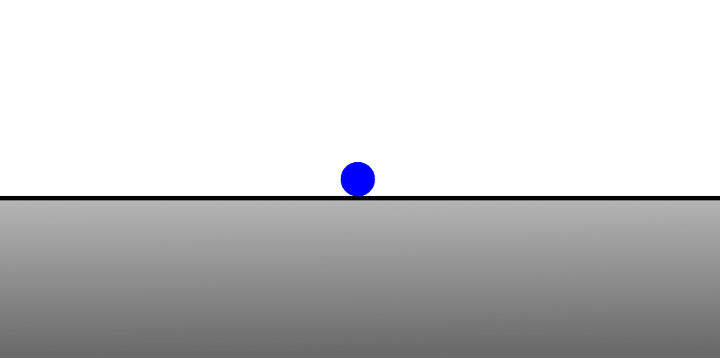
\includegraphics[height=1.3in]{NeutralEquilibirum}
        \label{Figure:StabilityBAH:Neutral}
    }
    \hfill
    \subfloat[No equilibrium (no steady-state)]{
        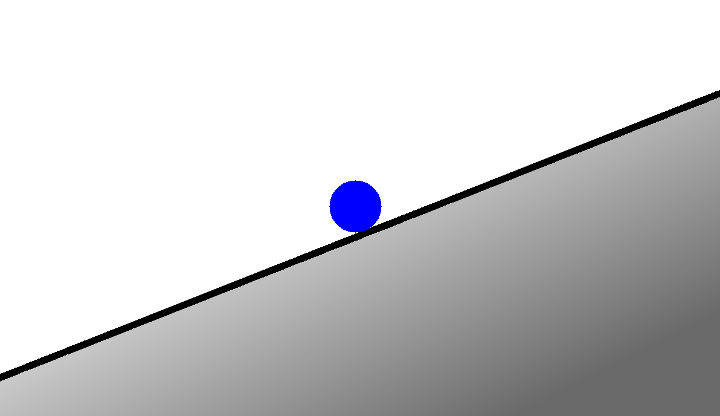
\includegraphics[height=1.3in]{NoEquilibirum}
        \label{Figure:StabilityBAH:None}
    }\\[3em]
    %
    %
    \subfloat[Stable equilibrium][Stable equilibrium \vspace{1.5em}]{
        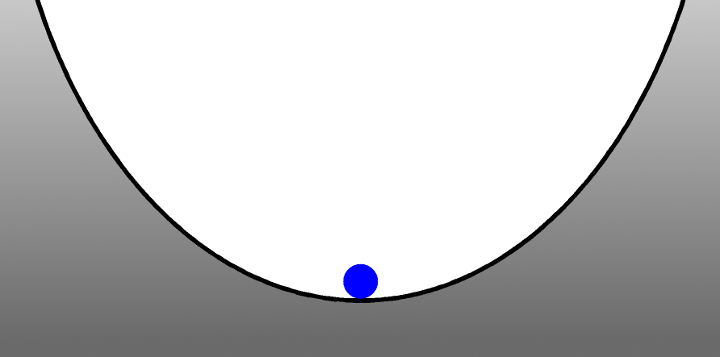
\includegraphics[height=1.3in]{Stable}
        \label{Figure:StabilityBAH:Stable}
    }
    \hfill
    \subfloat[Unstable equilibrium][Unstable equilibrium \vspace{1.5em}]{
        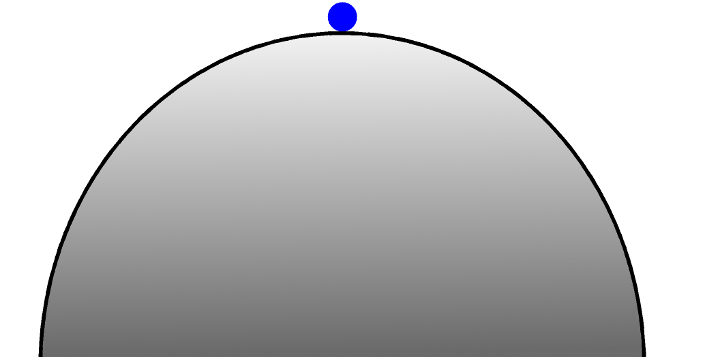
\includegraphics[height=1.3in]{Unstable}
        \label{Figure:StabilityBAH:Unstable}
    }\\[3em]
    %
    %
    \newcommand{\LUNS}{Linearly unstable, nonlinearly stable equilibrium}
    \newcommand{\LSNU}{Linearly stable, nonlinearly unstable  equilibrium}
    \subfloat[\LUNS][\LUNS\vspace{1.5em}]{
        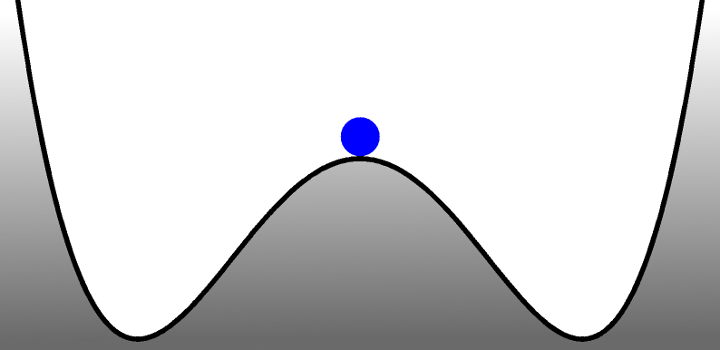
\includegraphics[height=1.3in]{LinearlyUnstableNonlinearlyStable}
        \label{Figure:StabilityBAH:LUNS}
    }
    \hfill
    \subfloat[\LSNU][\LSNU\vspace{1.5em}]{
        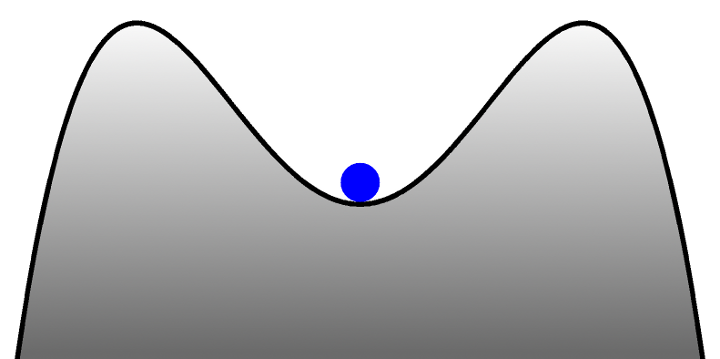
\includegraphics[height=1.3in]{LinearlyStableNonlinearlyUnstable}
        \label{Figure:StabilityBAH:LSNU}
    }
\end{figure}
A compound instability is one that incorporates two or more mechanisms that confound analysis; fundamental instabilities are the opposite.  Using a standard physical analogy, \cref{Figure:StabilityBAH:Stable} is a stable system while \cref{Figure:StabilityBAH:Unstable} is an example of a system with a static instability.

One aspect of the stability the above definitions do not discuss is the magnitude of the system perturbations.
The strength of the perturbation is important since it determines how much energy is imparted into the system and, therefore, how far the system will travel from its initial state.
The importance can be seen in \cref{Figure:StabilityBAH:LUNS,Figure:StabilityBAH:LSNU} where both systems exhibit different behavior depending how hard the system is ``hit.''
\Cref{Figure:StabilityBAH:LUNS} shows a linear instability while actually being nonlinearly stable with multiple equilibria.
\Cref{Figure:StabilityBAH:LSNU} exhibits linear stability while being nonliearly stable
These concepts are important to consider when looking at linear stability because the behavior beyond the system's linear boundary is technically \textit{terra incognita}.
Actually performing a nonlinear analysis, if possible, is the only surefire tool for assessing stability.


\subsubsection{Static Instabilities}
Static instabilities are characterized by either a pure steady-state analysis or an analysis that foresees dynamic feedback from the steady-state system.
The analysis tools used to derive stability boundaries for these instabilities will be discussed in \cref{Section:StabilityTheory}.

A flow excursion, also known as a Ledinegg instability, is the sudden drop in a steady flow rate to a lower, steady value.
This jump occurs when the pressure losses in a system decrease with increasing flow rate.
For a liquid undergoing phase change in a channel, there is a complex, internal relationship between the buoyancy, friction, and acceleration momentum terms that must be taken into account for steady flow.
If the flow is forced by external sources and the internal forces of the flow are not properly taken into account, then the pressure drop could rise with increasing flow; this is especially true for slightly sub-cooled flows entering a heated region where a sudden change in void fraction can have a large impact on the flow behavior with the system.

Fundamental relaxation instabilities occur when two or more flow regimes have state equilibriums close to each other.
For example, a bubbly flow that experiences a small change in flow rate could transition to the annular regime.
Then, the flow rate will experience an increase since annular flow has a relatively low pressure drop, and the flow regime transitions back to the bubbly regime.
Given the right situation, this cycle could continue ad infinitum.
The flow regime transitions act as a relaxation mechanism (in the dynamical system sense) that causes persistent, periodic behavior.

Chugging is an instability associated with the jetting of large vapor structures from a flow channel into larger space.
This instability typically occurs with low velocities and moderate void fractions \cite{tong_boiling_1997}.
A flowing liquid receiving heat may development large vapor bubbles in a coolant channel; this increases the flow rate due to the vapor-to-liquid ratio.
After the bubbles have been expelled, and possibly quenched, at the channel exit, the flow rate will return to the pre-slug rate.
As with the relaxation instability, this mechanism also has a periodic nature \cite{aritomi_geysering_1993}.



\subsubsection{Dynamic Instabilities}
Dynamic instabilities, unlike static, are inherently transient and primarily involve the transmission of information via waves.
As is discussed further in \cref{Chapter:Theory}, \THs systems typically possess a material (or density) wave and an acoustic (or pressure) wave.
For a non-ideal fluid, the acoustic wave's speed is primarily a function of the system's density and temperature while the material wave travels near the physical speed of the system.

Acoustic instabilities are typically of high frequency ($10$Hz--$10$kHz) and have been observed in various boiling regimes.
The acoustic waves were found to cause large pressure drop oscillations relative to steady-state values.
Even in situations where the lower frequency density waves were present, there was a clear superposition of high frequency acoustic waves with the material waves.
At high pressure-and-temperature water experiments, the acoustic waves reached frequencies that were clearly audible (so-called whistler modes).

Material wave instabilities are the most common in two-phase flow and are a highly physical phenomenon that occur from a complex coupling of \THs equations, constitutive relations, and geometry.
These waves have also been described as ``flow-void feedback instabilities'' for boiling systems \cite{neal_mechanisms_1967} and ``time-delay oscillations'' due to the relatively slow transmission of information at material speed \cite{boure_oscillatory_1966}.
Since the oscillation has its roots in the differing densities of a fluid's liquid and gas phases, vertical channel height (where the system pressure changes greatly with position), inlet conditions (thermodynamic and kinematic), and total heat transfer between the fluid and the surroundings are extremely important in the control and appearance of these flow oscillations.
It has been found that by increasing the system pressure these oscillations can be mitigated or eliminated since the density ratio of the competing phases approach one another as the pressure increases.

These material oscillations can lead to oscillations in the boiling heat transfer processes at the wall and results in a compound thermal instability.
The emphasis here is put on the highly variable nature of the two-phase heat transfer coefficient at the wall and how the information being propagated from the wall interacts with material wave oscillations.
The effects of this interaction can be as bad as an oscillating dry point in the channel with large temperature oscillations.



\subsubsection{Natural Circulation Instabilities}
There are two natural circulation instabilities of primary interest: flashing and compound natural circulation.
As mentioned in \cref{Section:RCCS}, flashing occurs when a high temperature liquid flows into a region of lower pressure such that it enters a saturated or superheated state and immediately bursts into a two-phase mixture.
This mechanism is a primary cause of material wave instabilities in natural circulation loops at low pressures or long vertical channels.
This type of instability is currently under examination for one and two protypic fuel channels \cite{marcel_experimental_2009,marcel_experimental_2010}.

The final instability is the compound natural circulation instability.
This instability is the confluence of vertical channel heating, material wave oscillations (possibly due to flashing), chugging phenomenon, and flow regime transitions.
Since the system's flow rate is not subject to any mechanical head contributions, all of these instabilities can occur concurrently and must be carefully analyzed to discern which of the mechanisms are present and which is dominate.
These instabilities are extremely important for all types of nuclear reactors and are under continuously under investigation \cite{dauria_characterization_1990,aritomi_fundamental_1992,yun_two-phase_2005}.

\begin{table}
    \centering
    \caption[Summary of static flow instabilities]{Summary of static flow instabilities due to \cite{boure_review_1973}}
    \label{Table:StaticInstabilities}
    \rowcolors{2}{}{Gray}
    \setstretch{1.05}
    \renewcommand{\arraystretch}{1.4}
    {\small
    \hyphenation{Transition}
    \hyphenation{Relaxation}
    \begin{tabular}{>{\centering}p{1.15in} >{\centering}p{1.1in}  >{\raggedright}p{1.4in}  >{\raggedright\arraybackslash}p{1.5in} }
        \toprule
        \multicolumn{1}{c}{\textbf{Name}}      & \multicolumn{1}{c}{\textbf{Class}} & 
        \multicolumn{1}{c}{\textbf{Mechanism}} & \multicolumn{1}{c}{\textbf{Characteristics}}\\\midrule
        % --------------------------------------------------------------------------------- 
        Flow excursion                     & Fundamental            & 
                \LedineggCriterion & Sudden, large flow change to a new, stable state \\
        % ---------------------------------------------------------------------------------
        Boiling crisis                     & Fundamental            & 
                Ineffective cooling & Wall temperature excursion and flow oscillation \\
        % ---------------------------------------------------------------------------------
        Flow Regime  Transition             & Fundamental Relaxation & 
                Varying \Delta{P} between regimes            & Cyclic flow pattern transitions and flow rate variations \\
        % ---------------------------------------------------------------------------------
        Bumping, geysering, or    chugging & Compound    Relaxation & 
                Periodic adjustment of metastable conditions & Periodic superheat and violent evaporation \\
    \bottomrule
    \end{tabular}
    }
\end{table}
\begin{table}
    \centering
    \caption[Summary of dynamic flow instabilities]{Summary of dynamic flow instabilities due to \cite{boure_review_1973}}
    \label{Table:DynamicInstabilities}
    \rowcolors{2}{}{Gray}
    \setstretch{1.05}
    \renewcommand{\arraystretch}{1.4}
    {\small
    \hyphenation{Compount}
    \hyphenation{Relaxation}
    \begin{tabular}{>{\centering}p{1.1in} >{\centering}p{1.1in} >{\raggedright}p{1.55in} >{\raggedright\arraybackslash}p{1.55in} }
        \toprule
        \multicolumn{1}{c}{\textbf{Name}}      & \multicolumn{1}{c}{\textbf{Class}} & 
        \multicolumn{1}{c}{\textbf{Mechanism}} & \multicolumn{1}{c}{\textbf{Characteristics}}\\\midrule
        % --------------------------------------------------------------------------------- 
        Acoustic  Oscillations  & Fundamental & Resonance of pressure waves & 
                High frequency oscillations near the acoustic speeds\\
        % ---------------------------------------------------------------------------------
        Density Wave  Oscillations  & Fundamental & Coupled mass, momentum, and energy feedback & 
                Low frequency oscillations near the material speed\\
        % ---------------------------------------------------------------------------------
        Thermal  Oscillations  & Compound & Variable heat transfer coefficient interacting with flow & 
                Occurs during film boiling \\
        % ---------------------------------------------------------------------------------
        BWR  Instability &  Compound & Hydraulic-neutronic coupling & 
                Strong only for a small fuel time constant and low pressure\\
        % ---------------------------------------------------------------------------------
        Parallel  Channel  Instability & Compound & Interaction among parallel channels & 
                Various modes of flow redistribution\\
        % ---------------------------------------------------------------------------------
        Pressure drop  Oscillations & Secondary Compound& 
                Flow excursions initiate interactions between channels and compressible volumes & 
                        Very low frequency, periodic process\\
    \bottomrule
    \end{tabular}
    }
\end{table}
\begin{table}
    \centering
    \caption[Effects of parametric variation on instability]
            {Effects of parametric variation on instability for a flow entering a vertical channel sub-cooled or saturated 
             due to \cite{durga_prasad_review_2007}}
    \label{Table:ParametericEffects}
    \rowcolors{2}{}{Gray}
    \setstretch{1.05}
    \renewcommand{\arraystretch}{1.5}
    {\small
    \hyphenation{Transition}
    \hyphenation{Relaxation}
    \begin{tabular}{>{\centering}p{1.6in} >{\raggedright}p{1.3in} >{\raggedright\arraybackslash}p{2.8in}}
        \toprule
        \multicolumn{1}{c}{\textbf{Parameter Increased}}  & \multicolumn{1}{c}{\textbf{Effect}} & 
        \multicolumn{1}{c}{\textbf{Reason}}\\\midrule
        % --------------------------------------------------------------------------------- 
        System pressure & Stability increases & Phase density difference lessens thus reducing the gravitational head gain. \\
        % ---------------------------------------------------------------------------------
        Mass flow rate  & Stability increases & Critical power for oscillation generation increases and avoids chugging.\\
        % ---------------------------------------------------------------------------------
        Inlet sub-cooling& Destabilizes at small sub-coolings but stabilizes otherwise &
                For small sub-coolings,due to significant response delay in void formation with an increase in transit time.
                Otherwise, it reduces void fraction and increases non-boiling length.\\
        % ---------------------------------------------------------------------------------
        Inlet resistance & Stability increases & Increases the single phase friction which has a damping effect upstream.\\
        % ---------------------------------------------------------------------------------
        Exist resistance & Stability reduces   & Increases two-phase friction which amplifies instabilities upstream\\
        % ---------------------------------------------------------------------------------
        Riser height     & Stability reduces   & 
                Increases two-phase gravitational pressure drop and phase transition as static head decreases\\
    \bottomrule
    \end{tabular}
    }
\end{table}

